\documentclass[11pt]{article}
\usepackage{amssymb}
\usepackage{amsthm}
\usepackage{enumitem}
\usepackage{amsmath, physics}
\usepackage{bm}
\usepackage{adjustbox}
\usepackage{mathrsfs}
\usepackage{graphicx}
\usepackage{siunitx}
\usepackage[mathscr]{euscript}

\title{\textbf{Solved selected problems of Classical Electrodynamics - Hans Ohanian}}
\author{Franco Zacco}
\date{}

\addtolength{\topmargin}{-3cm}
\addtolength{\textheight}{3cm}

\newcommand{\N}{\mathbb{N}}
\newcommand{\Z}{\mathbb{Z}}
\newcommand{\Q}{\mathbb{Q}}
\newcommand{\R}{\mathbb{R}}
\newcommand{\diam}{\text{diam}}
\newcommand{\cl}{\text{cl}}
\newcommand{\bdry}{\text{bdry}}
\newcommand{\inter}{\text{int}}
\newcommand{\uvi}{\bm{i}}
\newcommand{\uvj}{\bm{j}}
\newcommand{\uvk}{\bm{k}}
\newcommand{\hatx}{\bm{\hat{x}}}
\newcommand{\haty}{\bm{\hat{y}}}
\newcommand{\hatz}{\bm{\hat{z}}}
\newcommand{\hatrho}{\bm{\hat{\rho}}}
\newcommand{\hatphi}{\bm{\hat{\phi}}}
\newcommand{\hatr}{\bm{\hat{r}}}
\newcommand{\hatn}{\bm{\hat{n}}}
\newcommand{\hattheta}{\bm{\hat{\theta}}}
\newcommand{\sci}[1]{\times 10^{#1}}
\newcommand\numberthis{\addtocounter{equation}{1}\tag{\theequation}}

\theoremstyle{definition}
\newtheorem*{solution*}{Solution}
\renewcommand*{\proofname}{\bf{Solution}}

\begin{document}
\maketitle
\thispagestyle{empty}

\section*{Chapter 6 - The Theory of Special Relativity}

\subsection*{Problems}
\begin{proof}{\textbf{4.}}
\begin{itemize}
\item [(a)] Let the time interval between the birth of the blob at $Q$ and its
arrival at $P$ be $\Delta t_0$.\\
The time it takes for the light to arrive to the Earth from the birth of the
blob at $Q$ is
\begin{align*}
    \Delta t_{Q} = \frac{QO}{c}
\end{align*}
On the hand, the blob moves a distance $QP = V \Delta t_0$ towards the earth 
if we assume the angle is small.
So the time it takes for the light emitted at $P$ to reach the earth, assuming
we started measuring the time when the blob was born, is
\begin{align*}
    \Delta t_{P} = \frac{QO - QP}{c} + \Delta t_0
\end{align*}
Then the time interval between the reception at the Earth of the light emitted
at $Q$ and the light emitted at $P$ is
\begin{align*}
    \Delta t &= \Delta t_{P} - \Delta t_{Q} \\
    &= \frac{QO - QP}{c} + \Delta t_0 - \frac{QO}{c}\\
    &= \Delta t_0 -\frac{V\Delta t_0}{c}\\
    &= (1 - V)\Delta t_0
\end{align*}
Where we assumed that $c = 1$.

\cleardoublepage
\item [(b)] We note that $\sin \theta' = PP' / OP$ but if we assume the angle
is small then we have that
\begin{align*}
    PP' = \theta' OP
\end{align*}
So, if we assume that $Q$ and $P$ are not too far appart, then the apparent
transverse speed is given by
\begin{align*}
    \frac{PP'}{\Delta t} = \frac{\theta' OP}{(1 - V)\Delta t_0}
    = \frac{OP}{QP}\frac{\theta' V}{1 - V}
\end{align*}
Where we used that $\Delta t_0 = QP / V$.\\
Let us assume that $OP = 5~Gly$, $QP = 500~Mly$, $V = 0.99 c$
($99\%$ of the speed of light) and $\theta'= 0.1^\circ = 0.0017~rad$ then
\begin{align*}
    \frac{PP'}{\Delta t} = \frac{5\sci{9}}{1\sci{6}}\frac{0.0017\cdot0.99}{1 - 0.99}
    = 1.68 
\end{align*}
\end{itemize}
\end{proof}

\cleardoublepage
\begin{proof}{\textbf{5.}}
\begin{itemize}
\item [(a)] By integration we note that
\begin{align*}
    \int_{P_0}^P  dP &\leq c^2\int_{\rho_0}^\rho d\rho\\
    P - P_0 &\leq c^2 (\rho - \rho_0)\\
    P &\leq P_0 + c^2 (\rho - \rho_0)
\end{align*}

\item [(b)] The pressure in neutron-star material is
$P_0 = 1.22\sci{34}~g/cm \cdot s^2$ at a density of
$\rho_0 = 4.6\sci{14}~g/cm^3$.\\
Then, the pressure at a density $\rho = 10^{20} g/cm^3$ has the following
upper bound
\begin{align*}
    P &\leq 1.22\sci{34} + (10^{20} - 4.6\sci{14})\cdot (3\sci{10})^2\\
    &\leq 9\sci{40}~g/cm \cdot s^2
\end{align*}
If we set $\rho = 10^{30}~g/cm^3$ then $P$ has the following upper bound
\begin{align*}
    P &\leq 1.22\sci{34} + (10^{30} - 4.6\sci{14})\cdot (3\sci{10})^2\\
    &\leq 9\sci{50}~g/cm \cdot s^2
\end{align*}
\end{itemize}
\end{proof}

\cleardoublepage
\begin{proof}{\textbf{10.}}
To compute $a_x'$ we need to take the derivative of $u_x'$ with respect to $t'$
as follows
\begin{align*}
    a_x' = \frac{du_x'}{dt'}
    &= \dv{t'}(\frac{u_x - V}{1 - u_x V})\\
    &= \dv{t}{t'}\dv{t}(\frac{u_x - V}{1 - u_x V})\\
    &= \frac{dt}{\gamma (dt - Vdx)}\dv{t}(\frac{u_x - V}{1 - u_x V})\\
    &= \frac{\sqrt{1 - V^2}}{1 - u_xV}
    \bigg(\frac{a_x}{1 - u_x V} + \frac{(u_x - V)a_xV}{(1 - u_xV)^2}\bigg)\\
    &= a_x\frac{\sqrt{1 - V^2}}{1 - u_xV}
    \bigg(\frac{1 - u_xV + (u_xV - V^2)}{(1 - u_xV)^2}\bigg)\\
    &= a_x\frac{(1 - V^2)^{3/2}}{(1 - u_xV)^3}
\end{align*}
In the same way, for $a_y'$ we have that
\begin{align*}
    a_y' = \frac{du_y'}{dt'}
    &= \dv{t}{t'}\dv{t}(u_y\frac{\sqrt{1 - V^2}}{1 - u_x V})\\
    &= \frac{\sqrt{1 - V^2}}{1 - u_xV}
    \bigg(\frac{a_y\sqrt{1 - V^2}}{1 - u_x V}
    + \frac{a_xV (u_y\sqrt{1 - V^2})}{(1 - u_xV)^2}\bigg)\\
    &= \frac{a_y(1 - V^2)}{(1 - u_x V)^2}
    + \frac{a_xu_yV(1 - V^2)}{(1 - u_xV)^3}
\end{align*}
And finally, for $a_z'$
\begin{align*}
    a_z' = \frac{du_z'}{dt'}
    &= \dv{t}{t'}\dv{t}(u_z\frac{\sqrt{1 - V^2}}{1 - u_x V})\\
    &= \frac{\sqrt{1 - V^2}}{1 - u_xV}
    \bigg(\frac{a_z\sqrt{1 - V^2}}{1 - u_x V}
    + \frac{a_xV (u_z\sqrt{1 - V^2})}{(1 - u_xV)^2}\bigg)\\
    &= \frac{a_z(1 - V^2)}{(1 - u_x V)^2}
    + \frac{a_xu_zV(1 - V^2)}{(1 - u_xV)^3}
\end{align*}
\end{proof}

\cleardoublepage
\begin{proof}{\textbf{11.}}
\begin{itemize}
\item [(a)] We know from problem 10 that
\begin{align*}
    a_x = (1 - V^2)^{3/2} \frac{a'_x}{(1 - Vu'_x)^3}
\end{align*}
Since at the frame of the spaceship $u'_x = 0$ and $a_x = dV/dt$ then
\begin{align*}
    \dv{V}{t} = (1 - V^2)^{3/2} a'_x
\end{align*}
So by integration we have that
\begin{align*}
    \int_{0}^V (1 - V^2)^{-3/2}~dV &= \int_0^t a'_x ~dt\\
    \frac{V}{\sqrt{1 -V^2}} &= a'_x t
\end{align*}
Also, since $u'_x = 0$ we have that $u_x = V$ and hence
\begin{align*}
    \frac{u_x}{\sqrt{1 -u_x^2}} &= a'_x t\\
    u_x^2 &= (a'_x t)^2(1 - u_x^2)\\
    u_x^2(1 + (a'_x t)^2) &= (a'_x t)^2\\
    u_x^2 &= \frac{(a'_x t)^2}{1 + (a'_x t)^2}\\
    \dv{x}{t} &= \frac{a'_x t}{\sqrt{1 + (a'_x t)^2}}
\end{align*}
Then by integration again we have that
\begin{align*}
    \int_0^x dx &= a'_x \int_0^t \frac{t}{\sqrt{1 + (a'_x t)^2}}~dt\\
    x &= a'_x \bigg[\frac{\sqrt{1 + (a'_x t)^2}}{(a'_x)^2} - \frac{1}{(a'_x)^2}\bigg]\\
    x &= \frac{1}{a'_x}[\sqrt{1 + (a'_x t)^2} - 1]
\end{align*}

\item [(b)] When $V \ll 1$ we see that
\begin{align*}
    a'_x t = \frac{V}{\sqrt{1 - V^2}} \approx V
\end{align*}
So $a'_x t \ll 1$. Then, we can approximate the worldline equation using the
binomial approximation as follows
\begin{align*}
    x &\approx \frac{1}{a'_x}\bigg[1 + \frac{(a'_x t)^2}{2} - 1\bigg]
    =\frac{1}{2}a'_x t^2
\end{align*}
\end{itemize}
\end{proof}

\cleardoublepage
\begin{proof}{\textbf{12.}}
\begin{itemize}
\item [(a)] Let a particle move with speed $u'$ along a straight line in the
$x'$-$y'$ plane, the direction of the motion of the particle makes an angle
$\theta'$ with the $x'$ axis.\\
The components of the velocity in each direction in the $x'y'z'$ reference
frame are
\begin{align*}
    u'_x = u'\cos\theta' \qquad
    u'_y = u'\sin\theta'
\end{align*}
Then, the velocity components in the $xyz$ reference frame are
\begin{align*}
    u_x &= \frac{u'_x + V}{1 + u'_xV}
    = \frac{u'\cos\theta' + V}{1 + u'\cos\theta' V}\\
    u_y &= u'_y \frac{\sqrt{1 - V^2}}{1 + u'_x V}
    =  \frac{u'\sin\theta'\sqrt{1 - V^2}}{1 + u'\cos\theta' V}
\end{align*}
Also, $u_x$ and $u_y$ are related by $\tan \theta = u_y /u_x$ where $\theta$
is the angle the velocity $u$ makes with the $x$-axis, so
\begin{align*}
    \tan\theta = \frac{u_y}{u_x}
    = \frac{\frac{u'\sin\theta'\sqrt{1 - V^2}}{1 + u'\cos\theta' V}}
    {\frac{u'\cos\theta' + V}{1 + u'\cos\theta' V}}
    =\frac{u'\sin\theta'\sqrt{1 - V^2}}{u'\cos\theta' + V}
\end{align*}

\item [(b)] Suppose that a source at the origin of the $x'y'z'$ reference frame
emits particles in all directions.\\
If $V\to 1$ then for any angle $\theta' \in [0, 2\pi]$ we see that
\begin{align*}
    \lim_{V\to 1} \tan\theta
    = \lim_{V\to 1} \frac{u'\sin\theta'\sqrt{1 - V^2}}{u'\cos\theta' + V}
    = 0
\end{align*}
This is because $\sin\theta'$ becomes 0 at $\theta' = 0, \pi$ and $2\pi$,
making the limit 0 but the denominator is never 0 since $V\to 1$.\\
If $\sin\theta' \neq 0$ the limit also goes to 0 since $\sqrt{1 -V^2} \to 0$
as $V \to 0$.\\
So in any case the limit goes to 0.\\
Therefore, must be that $\theta = \pi n$ where
$n \in \Z$, so from the $xyz$ reference frame the particles form two narrow
beams in the forward direction ($\theta = 0, 2\pi, 4\pi, ...$) and 
in the backward direction ($\theta = \pi, 3\pi, 5\pi, ...$).
\end{itemize}
\end{proof}

\cleardoublepage
\begin{proof}{\textbf{19.}}
Let a spaceship leave Earth on a excursion to Barnard's star. The position of
the spaceship as a function of time is
\begin{align*}
    x = \frac{c^2}{g}\bigg(\sqrt{1 + \frac{g^2t^2}{c^2}} - 1\bigg)
\end{align*}
Where $t$ is the time measured in the reference frame of the Earth, with
$t =0$ at the start of the trip, and $g = 981~cm/s^2$ is the acceleration of
the spaceship in its own reference frame.
\begin{itemize}
\item [(a)] Taking the time derivative of $x$ we have that
\begin{align*}
    v = \dv{x}{t} = \frac{c^2}{g}\frac{g^2 t}{c^2\sqrt{1 + \frac{g^2t^2}{c^2}}}
    = \frac{g t}{\sqrt{1 + \frac{g^2t^2}{c^2}}}
\end{align*}
\item [(b)] When 2 years have elapsed on Earth, then the moving clock on the
spaceship has elapsed
\begin{align*}
    \tau &= \int_0^{2~y} \sqrt{1 - v^2/c^2} ~dt\\
    \tau &= \int_0^{2~y} \sqrt{1 - \frac{g^2 t^2}{c^2 + g^2t^2}} ~dt\\
    \tau &= \int_0^{2~y} \sqrt{\frac{c^2 + g^2t^2 - g^2 t^2}{c^2 + g^2t^2}} ~dt\\
    \tau &= \int_0^{2~y} \frac{1}{\sqrt{1 + g^2t^2/c^2}} ~dt\\
    \tau &= \int_0^{6.3\sci{7}~s}\frac{1}{\sqrt{1 + (981)^2t^2/(3\sci{10})^2}} ~dt\\
    \tau &= 4.5\sci{7}~s \approx 1.42~years
\end{align*}
\item [(c)] When 2 years have been elapsed in the Earth then the position of
the spaceship is
\begin{align*}
    x &= \frac{(3\sci{10})^2}{981}
    \bigg(\sqrt{1 + \frac{(981)^2(6.3\sci{7})^2}{(3\sci{10})^2}} - 1\bigg)
    = 1.183\sci{18}~cm
\end{align*}
The light needs to travel back to Earth the distance we just computed and since
the speed of light is the same for any observer, the time it takes for the radio
signal to reach the Earth is
\begin{align*}
    t = \frac{x}{c} = \frac{1.183\sci{18}}{3\sci{10}} = 39133333.3~s 
    = 1.24~years
\end{align*}
\item [(d)] We know that the velocity of the spaceship at the moment of sending
the radio signal is
\begin{align*}
    v = \frac{981 \cdot 6.3\sci{7}}{\sqrt{1 + \frac{(981)^2(6.3\sci{7})^2}{(3\sci{10})^2}}}
    = 26988436025.48~cm/s
\end{align*}
Since the signal is emitted with a frequency of $1\sci{9}~Hz$ in the reference
frame of the spaceship (the source), then the frequency at the arrival on Earth
will be
\begin{align*}
    \nu = \nu_0\sqrt{1 - v^2/c^2} = 1\times 10^9 \sqrt{1 - (0.899)^2} 
    = 4.37\sci{8}~Hz
\end{align*}
\end{itemize}
\end{proof}

\cleardoublepage
\begin{proof}{\textbf{20.}}\\
We see that the instantaneous velocities of each clock are
\begin{align*}
    V_1(t) = \dv{x}{t} = V_0 \quad\text{and}\quad V_2(t) = \dv{x}{t} = a_0t
\end{align*}
Then the proper time on the first clock (following a straight worldline) is
\begin{align*}
    \Delta \tau_1
    = \int_{t_A}^{t_B}\sqrt{1 - V_0^2}~dt
    = t_B\sqrt{1 - V_0^2}
\end{align*}
Where we used that $t_A = 0$.\\
For the second clock, following a curved worldline we have that
\begin{align*}
    \Delta \tau_2
    &= \int_{t_A}^{t_B}\sqrt{1 - a_0^2t^2}~dt\\
    &= \bigg[\frac{a_0t\sqrt{1 - a_0^2t^2} + \arcsin(a_0t)}{2a_0}\bigg]_0^{t_B}\\
    &= \frac{1}{2}t_B\sqrt{1 - a_0^2t_B^2} + \frac{\arcsin(a_0t_B)}{2a_0}
\end{align*}
We notice that when $t = t_B$ we have that $x_B = V_0 t_B$ and
$x_B = \frac{1}{2}a_0 t_B^2$ so
\begin{align*}
    \frac{1}{2}a_0 t_B^2 &= V_0 t_B\\
    t_B &= \frac{2V_0}{a_0}
\end{align*}
Where we used that the worldlines have the same value at $t=t_B$.\\
Then the proper time equations become
\begin{align*}
    \Delta \tau_1
    = \frac{2V_0}{a_0}\sqrt{1 - V_0^2}
    \qquad
    \Delta \tau_2
    = \frac{V_0}{a_0}\sqrt{1 - 4V_0^2} + \frac{\arcsin(2V_0)}{2a_0}
\end{align*}
Below, we plotted the real part of both equations for different values of $V_0$
\begin{center}
    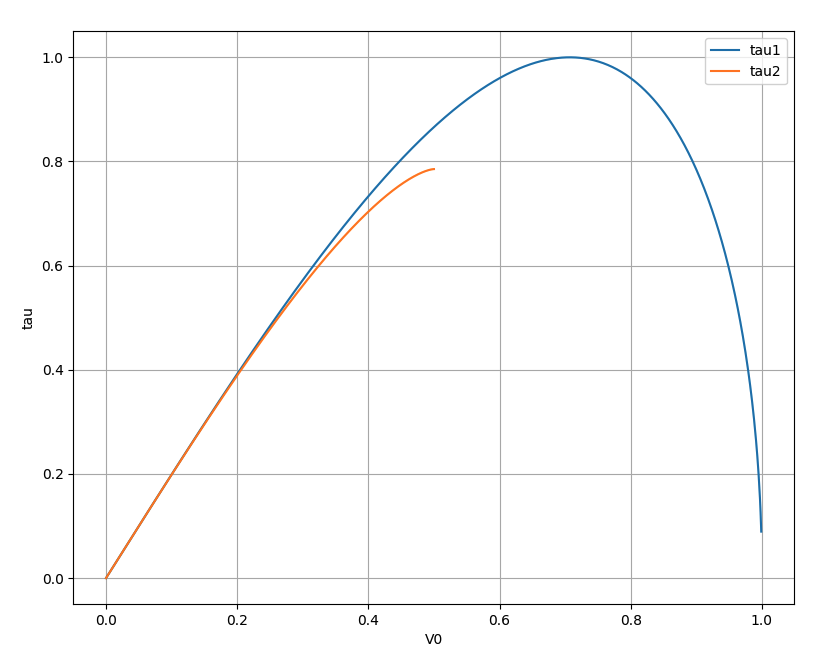
\includegraphics[scale=0.35]{ch6-20.png}
\end{center}
We notice that $\Delta \tau_1$ is always bigger than $\Delta \tau_2$ so the
clock following the straight worldline shows the longer proper time.
\end{proof}

\cleardoublepage
\begin{proof}{\textbf{21.}}\\
Let us consider a reference frame in which the free particle is at rest, then
in this reference frame from the event $A$ to the event $B$ the proper time
is
\begin{align*}
    \Delta\tau_1 = \int_{t_A}^{t_B} \sqrt{1 - 0^2}~dt
    = \int_{t_A}^{t_B} dt = \Delta t
\end{align*}
From this reference frame, taking a spacetime diagram in which the position of
the particle matches the origin, the worldline of the particle is
a line along the $t$-axis. So any other worldline between the events $A$ and
$B$ must be a line in which the particle is not free, since it needs to move
away from the $t$-axis and then come back. For such a worldline the proper time
is
\begin{align*}
    \Delta\tau_{2} = \int_{t_A}^{t_B} \sqrt{1 - V(t)^2}~dt
\end{align*}
Since $V(t) \leq 1$ then $ \sqrt{1 - V(t)^2} \leq 1$. Also, in between the 
events $A$ and $B$ there must be an interval where $V(t) \neq 0$ otherwise
we would be following the free particle worldline, suppose between the events
$C$ and $D$ we have that $V(t) \neq 0$ then we have that
$\sqrt{1 - V(t)^2} < 1$ in that interval. \\
Therefore
\begin{align*}
    \Delta\tau_2 = \int_{t_A}^{t_B} \sqrt{1 - V(t)^2}~dt
    < \int_{t_A}^{t_B} dt = \Delta\tau_1
\end{align*}
Hence, the proper time of a free particle is the largest.
\end{proof}

\cleardoublepage
\begin{proof}{\textbf{22.}}\\
Let us consider the star Capella at a distance of 46 light-years from Earth.
An astronaut wants to travel from Earth to Capella in a time no more than 
20 years as reckoned by clocks aboard his spaceship.\\
Seen from Earth the astronaut moves with a velocity
$$V = \frac{\Delta x}{\Delta t}$$
We want that the clock aboard the spaceship measures at the end of
the trip $\Delta \tau = 20$ years and we know that $\Delta \tau$ and $\Delta t$
are related by
\begin{align*}
    \Delta t = \frac{\Delta \tau}{\sqrt{1 - V^2}}
\end{align*}
So the spaceship needs to travel at a speed of
\begin{align*}
    V = \frac{\Delta x}{\Delta t}
    &= \frac{\Delta x\sqrt{1 - V^2}}{\Delta \tau}\\
    V^2 &= \frac{\Delta x^2}{\Delta \tau^2}(1 - V^2)\\
    V^2 + \frac{\Delta x^2}{\Delta \tau^2}V^2
    &= \frac{\Delta x^2}{\Delta \tau^2}\\
    V &= \frac{\Delta x}{\Delta \tau}
    \bigg(1 + \frac{\Delta x^2}{\Delta \tau^2}\bigg)^{-1/2}
\end{align*}
Replacing values
\begin{align*}
    V &= \frac{46 \text{ light-years}}{20 \text{ years}}
    \bigg(1 + \frac{(46 \text{ light-years})^2}{(20 \text{ years})^2}\bigg)^{-1/2}\\
    &= 0.917~c
\end{align*}
Finally, a clock on Earth would measure
\begin{align*}
    \Delta t = \frac{20\text{ years}}{\sqrt{1 - (0.917)^2}}
    = 50.13\text{ years}
\end{align*}

\end{proof}

\cleardoublepage
\begin{proof}{\textbf{25.}}\\
We know that the Earth moves around the Sun at a speed of $30~km/s$, if 
we assumee that the Earth is a perfect sphere of radius $6.4\sci{6}~m$ then 
the east-west diameter will be contracted by
\begin{align*}
    2R - 2R \sqrt{1 - \frac{V^2}{c^2}}
    = 2 \cdot 6400\cdot \bigg(1 - \sqrt{1 - \frac{30^2}{300000^2}}\bigg)
    = 0.064~m
\end{align*}
The length contraction is barely noticeable since the velocity of the Earth
is 0.01\% of the speed of light.\\
The transverse directions are not length contracted so, if the Earth has a
volume of
$$V = \frac{4}{3} \pi r^3 = \frac{4}{3} \pi 6400^3
= 1.09\sci{12}~km^3$$
Then from the sun the volume will be contracted by
\begin{align*}
    V - V \sqrt{1 - \frac{V^2}{c^2}}
    = 1.09\sci{12}\cdot\bigg(1 - \sqrt{1 - \frac{30^2}{300000^2}}\bigg)
    = 5450~km^3
\end{align*}
\end{proof}
\end{document}
